\chapter{Mean field theory for small world networks}

The previous chapter focused mainly on simulation results for ring-lattices and small-world networks. In this chapter we develop a mean
field (MF) theory for the WCM dynamics on a system of $N$ oscillators coupled according to small world networks as described by the
Watts Strogatz algorithm in section~\ref{smallworld}. We start by re-stating the dynamics rules and proceed to take the continuous
limit.

An oscillator is described by its discrete phase state, which can be imagined as a clock hand which abruptly jumps from noon to 4pm
then 8pm and back to noon. These jumps happen randomly but with a well defined average rate over time. When two oscillators interact,
this average rate of transition may change depending on the relative phase between the two units.

To describe the phase value and interactions, we adopt a convention: oscillators are arranged in a circle and numbered from 1 to $N$.
The superscripts then refer to the oscillators index. Subscripts denote a phase state from 1 to 3. Given a graph where nodes represent
phase oscillators labeled by $x$, the unit at position $x$ is described by its phase value

\begin{align}
    \phi^x = 2\pi (j-1)/3 \\
    j \in \{1,2,3\} \notag
\end{align}

\noindent where $j$ is the state of unit $x$. Since transitions can only occur in one direction, for a given unit at $x$, the
stochastic rate of transition from state $j$ to $j+1$ is written just as $\gamma^x_j$, and is given by the Arrhenius form:

\begin{equation}
    \gamma^x_j = \omega^x\exp\left[ a\frac{n^x_{j+1} - n^x_j}{n^x} \right] \qquad x=1,\dots, N
    \label{rate}
\end{equation}

\noindent where $\omega^x$ is its natural (uncoupled) frequency, $n^x_j$ is the count of how many of its neighbors are in state $j$,
and $n^x$ is its total number of neighbors.

Let the probability of finding the unit at $x$ in state $j$ be denoted by $p^x_j$. Since there are only three possible states we have
the restrictions $p^x_1+p^x_2+p^x_3=1$ for all $x$. The rate of change of the probabilities can be written in terms of the transition
rates $\gamma^x_j$, giving us $2N$ equations of motion:

\begin{align}
    \ddt{p}^x_1 &= \gamma^x_3(1 - p^x_1 - p^x_2) - \gamma^x_1 p^x_1 & \notag\\
    \ddt{p}^x_2 &= \gamma^x_1p^x_1 - \gamma^x_2 p^x_2 &x=1,\dots,N
    \label{eqmotion}
\end{align}

\noindent The first terms in the RHS of (\ref{eqmotion}) represent the fluxes of probability from oscillators in the previous state,
which can advance one phase state and increase the populations of oscillators in states 1 and 2 respectively. The second (negative)
terms represent the fluxes generated by the oscillator leaving the considered state, and thus reducing that states population.  This
dynamics occurs on small-world networks, which are generated following the Watts-Strogatz algorithm starting with a ring lattice.

A ring lattice is constructed by arranging $N$ oscillators in a circle, and then for each unit, add $K$ clock-wise connections to the
next $K$ units in the circle, resulting in a circular shape with $NK$ total edges. The result of this process for $N=12$ and $K=2$ can
be seen in figure~\ref{fig:ring} in chapter~\ref{chap:article}.

To generate a small-world network, the rewiring procedure considers each existing edge once, and with a probability $p$ it changes the
clockwise vertex of this edge by a randomly selected node in the network. If the randomly selected node would create an already
existing edge or a self-connection, no action is performed.

\section{Deriving the local average field}

By defining the fractions in the exponent of equation~(\ref{rate}) at a fixed time $t$ as

\begin{equation}
    \nu^x_j(t) \equiv \frac{n^x_j(t)}{n^x(t)}
\end{equation}

\noindent the transition rates are now written as

\begin{align}
    \gamma^x_j(t) = g^x\exp\left[ a(\nu^x_{j+1}(t) - \nu^x_j(t)) \right]
    \label{mfrate}
\end{align}

The quantity $\nu^x_j$
describes the fraction of sites which are connected to node $x$ that are in state $j$ and thus also satisfies
$\nu^x_1+\nu^x_2+\nu^x_3=1$.

In the continuous limit, the average values of $\nu$ will dictate the dynamics. This was done previously by substituting $\nu$ in
equation (\ref{mfrate}) by its average \cite{escaff2014arrays}, which is taken over independent realizations of the dynamics. The
average-field rate of transition becomes:

\begin{align}
    %\left< \gamma^x_j \right> = g^x \exp \left[ a \left( \left< \nu^x_{j+1} \right> - \left< \nu^x_j \right> \right) \right]
    \gamma^x_{j,MF} = g^x \exp \left[ a \left( \left< \nu^x_{j+1} \right> - \left< \nu^x_j \right> \right) \right]
    \label{gammaMF}
\end{align}

For regular rings the number of neighbors of every site is two times the interaction range ($n^x = 2K \quad \forall x$), but since we
are now dealing with rewired networks, $n^x$ becomes a random variable which assumes different values at each site with respect to the
different realizations over which we take the averages. Thus we proceed in the same way and define the mean field value of $\nu$ by
replacing the random variables $\nu^x$ and $\nu^x_j$ by their averages:

\begin{align}
    \nu^x_{j,MF}(t) = \frac{\left< n^x_j(t) \right>}{\left< n^x(t) \right>}
    \label{nuMF}
\end{align}

\noindent where the average is taken over independent realizations and \textit{not} over time. The master equations for the mean field
are obtained by replacing the instantaneous rates of transition by their average-field values in (\ref{eqmotion}).

\begin{align}
    \ddt{p^x_1} &= \gamma^x_{3,MF} (1-p^x_1-p^x_1) - \gamma^x_{1,MF} p^x_1 \notag \\
    \ddt{p^x_2} &= \gamma^x_{1,MF}  p^x_1 - \gamma^x_{2,MF} p^x_2
    \label{eqmotionMF}
\end{align}

We see that in order to have any hope of solving the set of equations~(\ref{nuMF})~to~(\ref{eqmotionMF}) we must be able to calculate
the averages of the random variables $n^x$ and $n^x_j$.

To do that, we define the dummy variable $D_{xx'}$, which indicates the presence (or absence) of a connection between nodes $x$ and
$x'$ in a graph. With this notation we can write the exact expressions for $n^x$ and $n^x_j$ in the discrete case. Let $D_{xx'}$ be
defined as

\begin{align}
    D_{xx'} = 
    \begin{cases}
        1 \qquad &\text{if the connection $x$,$x'$ exists}\\
        0 \qquad &\text{otherwise}
    \end{cases}
\end{align}

\noindent then, if the states of sites $x,x'$ are $j,j'$ respectively, we have:

\begin{align}
    n^x_j &= \sum\limits_{x'=1}^ND_{xx'}\delta_{jj'}(t) \notag\\[8pt]
    n^x &= \sum\limits_{x'=1}^ND_{xx'}
\end{align}

\noindent where $\delta_{jj'}$ is the usual Kronecker delta defined by $\delta_{jj'}=\begin{cases}1 \quad j=j'\\0 \quad j\neq
j'\end{cases}$, and thus $\left< \nu^x_j(t) \right>$ becomes

\begin{align}
    \left< \nu^x_j(t) \right> &= \frac{\sum\limits_{x'=1}^N\left< D_{xx'}\delta_{jj'}(t)\right>}{\sum\limits_{x'=1}^N\left< D_{xx'} \right>}
    \notag \\[8pt]
    \left< \nu^x_j(t) \right> &= \frac{\sum\limits_{x'=1}^N\left< D_{xx'}\right>\left<\delta_{jj'}(t)\right>}{\sum\limits_{x'=1}^N\left< D_{xx'} \right>}
\end{align}

\noindent Here we have assumed $\left< D_{xx'}\delta_{jj'}(t)\right> = \left< D_{xx'}\right>\left<\delta_{jj'}(t)\right>$ in order to
solve the proposed MF approximation. In words this means the state of site $x'$ depends on the state of site $x$ regardless of them
being coupled or not, but the strength of the coupling is modulated by the ``average connectivity'' value $\left< D_{xx'} \right>$.
This approximation becomes more accurate when the probability of rewiring $p$ is approaches zero, which is true for a large number of
networks in the small-world regime, as seen in figure~\ref{fig:small-world} of chapter~\ref{chap:article}. When $p=0$ we can restrict
the summation over the connected sites and recover the MF proposed by Escaff \textit{et al.}~\cite{escaff2014arrays}, making
$\delta_{jj'}$ truly independent from $D_{xx'}$.

The average $\left< \delta_{jj'}(t) \right>$ can now be identified with the probability of finding the site at $x'$ in state $j$ at
time $t$: $\left< \delta_{jj'}(t) \right> \equiv p^{x'}_j(t)$, and we are left with the task of calculating $\left< D_{xx'} \right>$.
In order to do this, we need a detailed description of the rewiring algorithm, which will ultimately dictate the connectivity of the
final graph. 

\subsection{Rewiring algorithm}

Arrange $N$ nodes in a circle and for each one connect it with an edge to the next $K$ clockwise nearest neighbors. Choose a starting
point and consider the edge to the \text{first} clockwise nearest neighbor. With probability $p$, swap the clockwise node that
constitutes this edge for a uniformly selected node on the entire network, except if the selected node is itself or if there is already
an edge between the new pair. Repeat this process for all the first clockwise nearest neighbors, and than go back to the starting
point. Repeat the process for all \textit{second} nearest neighbors this time, and than the \textit{third} and so on, until all the
$NK$ initial edges have been considered exactly once.

Let $d_{xx'}$ denote the distance between nodes $x$ and $x'$ in the one dimensional chain as illustrated in
figure~\ref{fig:ring-distance}. To calculate the average values $\left< D_{xx'} \right>$ we consider the two cases: \textbf{case
}$\mathbf{d_{xx'} \leq K}$ and \textbf{case} $\mathbf{d_{xx'} > K}$. If the initial distance between two nodes is less than $K$, than
by construction of the initial graph they start out connected. The condition that this connection exists in the final graph is that it
was never removed in the first place, or that it was removed and than subsequently reformed. Sites with $d_{xx'}>K$ start disconnected,
and thus the condition for it being present in the final graph is that some of it's vertices got rewired that way. With a little
deliberation on the rewiring procedure, one will agree that if the process produces any edge, then it cannot be broken in any of the
subsequent steps. Thus, the occurrence of any forming event between two nodes guarantees that connection will be present in the final
graph. Conversely, if an initial connection is not broken, it will remain on the final graph.

\begin{figure}
    \centering
    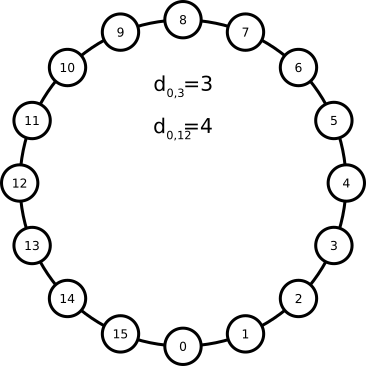
\includegraphics[width=0.40\textwidth]{fig/ring-distance.png}
    \caption{\label{fig:ring-distance}
        Definition of distance $d_{xx'}$ between sites $x$ and $x'$. The distance $d_{xx'}$ is considered on the one dimensional chain
        and does not take into account the connections that determine the coupling. This can be imagined as a periodic one dimensional
        system with interaction range $K$, which determines the coupling for the dynamics. Note that the periodicity leads to the
        distance between $x=0$ and $x'=12$ being 4 and \textit{not} $12-0=12$.
    }
\end{figure}

\subsection{Case $\mathbf{d_{xx'}>K}$:}



\begin{align}
    x
\end{align}
